\section{问题一的建模与求解：Y 染色体浓度与孕周、BMI 的关系模型}

\subsection{问题分析}

若直接对全部样本做横截面相关分析，Y 染色体浓度与孕周、BMI 的相关性均很弱（Pearson 相关系数分别为 0.127 与 $-0.151$）。这并非说明二者无关，而是因为数据为纵向面板数据，存在混杂：高 BMI 孕妇的 Y 浓度较低，而她们往往被安排在更晚的孕周检测，从而掩盖了孕周与 BMI 各自的真实效应。因此，必须用面板数据方法将``孕周效应''（组内）与``BMI 效应''（组间）分离。

\subsection{面板分解}

设第 $i$ 名孕妇在第 $j$ 次检测的 Y 浓度为 $Y_{ij}$，对应孕周为 $t_{ij}$。构造组内去均值：

\begin{equation}
  \tilde{Y}_{ij}=Y_{ij}-\bar{Y}_i,\qquad \tilde{t}_{ij}=t_{ij}-\bar{t}_i,
\end{equation}

其中 $\bar{Y}_i,\bar{t}_i$ 为该孕妇各次检测的均值。固定效应回归

\begin{equation}
  \tilde{Y}_{ij}=\beta_1\,\tilde{t}_{ij}+\varepsilon_{ij}
\end{equation}

的斜率 $\beta_1$ 刻画了``同一孕妇内 Y 浓度随孕周的变化''。对组间（个体均值）做回归：

\begin{equation}
  \bar{Y}_i=\alpha+\beta_2\,B_i+\eta_i,
\end{equation}

其斜率 $\beta_2$ 刻画了``BMI 对个体平均浓度的影响''。

\subsection{结果与显著性检验}

计算结果如表~\ref{tab:p1} 所示。

\begin{center}
\begin{tabular}{lccc}
\toprule
\textbf{效应} & \textbf{系数} & \textbf{统计量} & \textbf{p 值} \\
\midrule
组内孕周（固定效应） & 0.00319 /周 & $t=24.26$ & $4.0\times 10^{-104}$ \\
组间 BMI & $-0.00222$ /BMI & $t=-4.05$ & $6.6\times 10^{-5}$ \\
\bottomrule
\end{tabular}
\captionof{table}{问题一面板分解结果}
\label{tab:p1}
\end{center}

由表~\ref{tab:p1} 可知：

\begin{itemize}
  \item 组内 Y 浓度与孕周的相关系数高达 $0.594$，孕周效应高度显著（$p<10^{-100}$），即同一孕妇 Y 浓度随孕周约每周上升 $0.32$ 个百分点；
  \item BMI 在个体之间表现为显著负效应（$p<10^{-4}$），BMI 每升高 1，Y 浓度约下降 $0.22$ 个百分点，符合胎儿游离 DNA 随母体 BMI 升高而被稀释的生理规律\cite{ref2,ref4}。
\end{itemize}

图~\ref{fig:q1_scatter} 直观展示了组内去均值后 Y 浓度随孕周的强上升关系，以及组间 Y 浓度随 BMI 的下降关系。

\begin{figure}[H]
  \centering
  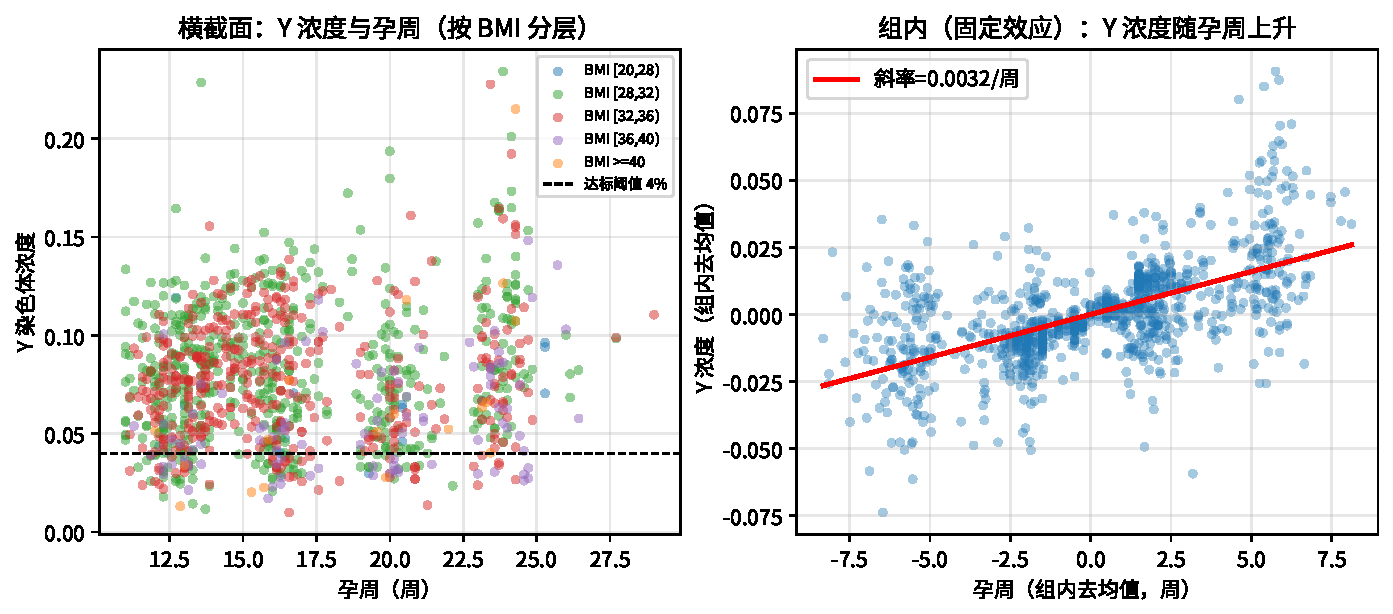
\includegraphics[width=0.9\textwidth]{../figures/fig1_1_scatter_within.pdf}
  \caption{横截面 Y 浓度随孕周的变化（按 BMI 分层，左）与组内去均值后 Y 浓度随孕周上升（右）}
  \label{fig:q1_scatter}
\end{figure}

\begin{figure}[H]
  \centering
  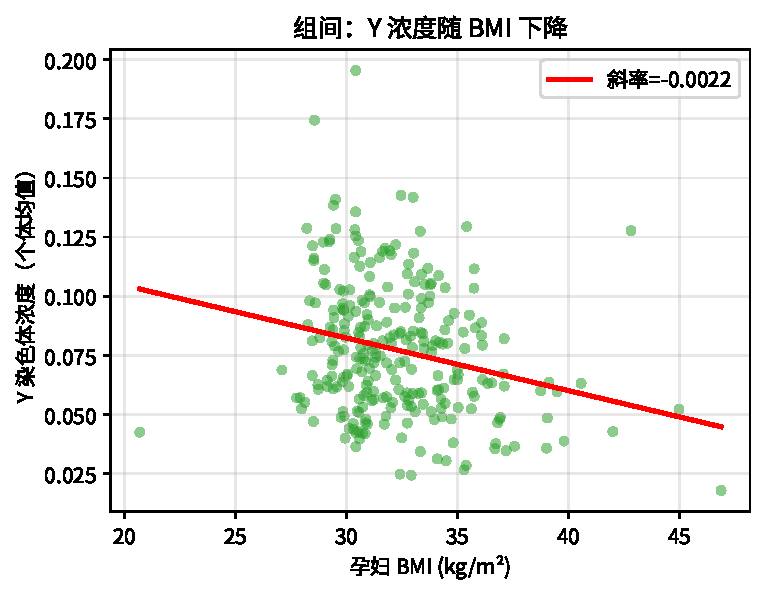
\includegraphics[width=0.62\textwidth]{../figures/fig1_2_between_bmi.pdf}
  \caption{组间 Y 浓度个体均值随 BMI 下降}
  \label{fig:q1_between}
\end{figure}

\subsection{混合效应关系模型}

将组内与组间效应统一到混合效应模型中：

\begin{equation}
  Y_{ij}=\beta_0+\beta_1 t_{ij}+\beta_2 B_i+u_i+\varepsilon_{ij},
\end{equation}

其中 $u_i\sim N(0,\sigma_u^2)$ 为个体随机截距。模型估计结果（见表~\ref{tab:p1_me}）为：

\begin{equation}
  Y=0.070+0.00313\,t-0.00138\,B+u_i+\varepsilon.
\end{equation}

\begin{center}
\begin{tabular}{lcccc}
\toprule
\textbf{项} & \textbf{系数} & \textbf{标准误} & \textbf{z 值} & \textbf{p 值} \\
\midrule
截距 $\beta_0$ & 0.070 & 0.016 & 4.31 & $<0.001$ \\
孕周 $\beta_1$ & 0.00313 & 0.00016 & 19.43 & $<0.001$ \\
BMI $\beta_2$ & $-0.00138$ & 0.00052 & $-2.65$ & 0.008 \\
\bottomrule
\end{tabular}
\captionof{table}{混合效应模型系数}
\label{tab:p1_me}
\end{center}

孕周效应与 BMI 效应在混合效应模型中均高度显著（$p<0.01$）。模型比较显示（AIC 分别为：线性 $-5059.26$、含交互 $-5059.09$、含交互与二次项 $-5077.36$），交互项与二次项均不显著，线性模型已能充分刻画关系，说明在检测窗口内 Y 浓度随孕周近似线性上升。

\begin{figure}[H]
  \centering
  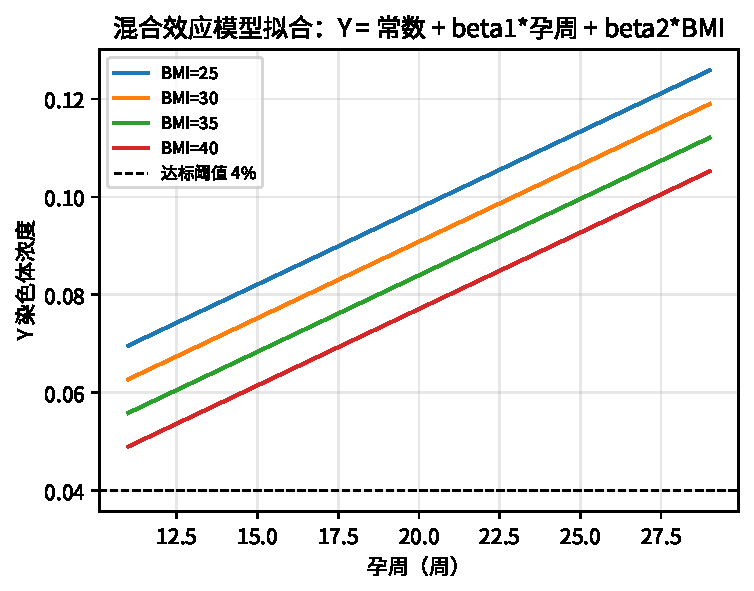
\includegraphics[width=0.62\textwidth]{../figures/fig1_3_fitted.pdf}
  \caption{混合效应模型拟合：不同 BMI 下 Y 浓度随孕周的线性轨迹}
  \label{fig:q1_fitted}
\end{figure}

综上，Y 染色体浓度随孕周线性上升、随 BMI 线性下降，两者关系均显著；横截面的弱相关是混杂造成的假象，须用面板/混合效应方法才能识别真实关系。
